116. а) $$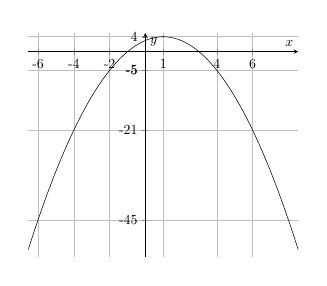
\begin{tikzpicture}[scale=0.5]
\begin{axis}[
    axis lines = middle,
    grid=major,
    legend pos={south west},
    xlabel = {$x$},
    ylabel = {$y$},
    ymin=-55,
    ymax=5,
    xtick={-6,-4, -2,1,4,6,10},
    xticklabels={-6,-4, -2,1,4,6,8},
    ytick={-45,-21,-5,4,-5},
    yticklabels={-45,-21,-5,4,-5}            ]
\addplot[domain=-8:10, samples=100, color=black] {-x*x+2*x+3};
\end{axis}
\end{tikzpicture}$$\\
б) $$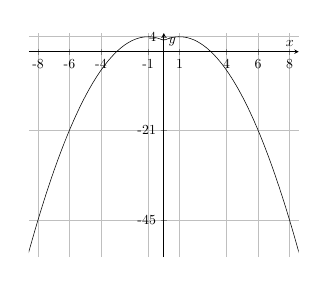
\begin{tikzpicture}[scale=0.5]
\begin{axis}[
    axis lines = middle,
    grid=major,
    legend pos={south west},
    xlabel = {$x$},
    ylabel = {$y$},
    ymin=-55,
    ymax=5,
    xtick={-8, -6,-4,-1, 1,4,6,8},
    xticklabels={-8,-6,-4,-1, 1,4,6,8},
    ytick={-45,-21,4},
    yticklabels={-45,-21,4}            ]
\addplot[domain=-10:10, samples=100, color=black] {-x*x+2*abs(x)+3};
\end{axis}
\end{tikzpicture}$$

ewpage
